% Time-stamp: <2016-06-10 12:57:54 chl>
\documentclass[20pt,landscape,dvips]{foils} 
% add 'draft' option above to exclude image when compiling
\usepackage[french]{babel}
\usepackage[utf8]{inputenc}  
\usepackage{csquotes} 
%\MakeOuterQuote{"}
\frenchspacing
\DecimalMathComma

\usepackage{latexsym}
\usepackage{amsmath,amssymb,amsfonts}
\usepackage{MnSymbol}
\usepackage{url}
\usepackage{graphicx}
%\usepackage[dvipsnames]{xcolor}
\usepackage{hyperref}
\usepackage{alltt}
\usepackage{pifont,manfnt}
\usepackage[dvipsnames,table]{xcolor}
\usepackage{subfig}
%\usepackage{enumerate}
%\usepackage{colortbl}
\usepackage{multirow,hhline}
\usepackage{cclicenses}
\setlength\parindent{0pt}
\hypersetup{colorlinks=true,citecolor=black,urlcolor=black,linkcolor=black}
\usepackage[style=verbose]{biblatex}
\bibliography{refs}

\newcommand{\highlight}[1]{\textcolor{Plum}{\bfseries #1}}
\newcommand{\remark}[1]{%
%\centerline{
\begin{center}
\framebox[.9\textwidth][t]{
\ding{46} 
\parbox[t]{.8\textwidth}{\small #1}}
\end{center}}

\DeclareMathOperator*{\inlaw}{\sim}
\newcommand{\iid}{\inlaw_{\text{i.i.d.}}}
%\newcommand{\iid}{\mathop{\mathrm{diag}}}
\newcommand{\pobs}{p_{\text{obs}}}

\reversemarginpar
\def\mark{\marginpar{\dbend}}

%\newcommand{\bm}[1]{\mbox{\boldmath{$#1$}}}
\renewcommand{\abstractname}{Summary}
\newcommand\bs{\char '134}   %  a backslash character for the \tt font
%\renewcommand\refname{Additional Readings}

% customize header/footer
\rightheader{}
% Note about the copyleft symbol:
% I use a custom reversed and circled "c" char because \textcopyleft in
% the textcomp package does not support sans serif font.
% Also, "c" is shifted horizontally by 1ex to align with the circle.
%\Restriction{\mbox{\raisebox{1.5ex}{\rotatebox{180}{\textcircled{c\kern.1ex}}} 2009}, \url{www.aliquote.org}}
% now I use the CC licence...
% \Restriction{\cc 2016 \VCRevision}
\Restriction{\cc 2016 Module 11 EESPE}

\title{Méthodes psychométriques en qualité de vie} 
\author{Christophe Lalanne\\EA 7334 REMES\\ Unité de Méthodologie des critères
  d’évaluation\\Université Paris-Diderot, Sorbonne Paris-Cité\\}
\date{
\includegraphics[height=18ex]{logo.eps}}

%%% This file has been generated by the vc bundle for TeX.
%%% Do not edit this file!
%%%
%%% Define Git specific macros.
\gdef\GITHash{f4328f7906d309e9224e3e5c2f7f36477f44e69f}%
\gdef\GITAbrHash{f4328f7}%
\gdef\GITParentHashes{136657e4877819e72dc9ebb2f209631a2a8d1057}%
\gdef\GITAbrParentHashes{136657e}%
\gdef\GITAuthorName{Christophe Lalanne}%
\gdef\GITAuthorEmail{ch.lalanne@gmail.com}%
\gdef\GITAuthorDate{2016-07-06 10:29:58 +0200}%
\gdef\GITCommitterName{Christophe Lalanne}%
\gdef\GITCommitterEmail{ch.lalanne@gmail.com}%
\gdef\GITCommitterDate{2016-07-06 10:29:58 +0200}%
%%% Define generic version control macros.
\gdef\VCRevision{\GITAbrHash}%
\gdef\VCAuthor{\GITAuthorName}%
\gdef\VCDateRAW{2016-07-06}%
\gdef\VCDateISO{2016-07-06}%
\gdef\VCDateTEX{2016/07/06}%
\gdef\VCTime{10:29:58 +0200}%
\gdef\VCModifiedText{\textcolor{red}{with local modifications!}}%
%%% Assume clean working copy.
\gdef\VCModified{0}%
\gdef\VCRevisionMod{\VCRevision}%


\begin{document}
\LogoOff
\maketitle
\rightfooter{\quad\textsf{\thepage}}



%---------------------------------------------------------------Slide-
\foilhead{Objectifs de l'atelier}

\begin{itemize}
\item Vue d'ensemble des techniques de développement, validation et analyse de
  questionnaires et de mesures patients ;
\item Outils statistiques de base : (1) théorie classique des tests et analyse
  de fidélité de mesure, (2) analyses factorielles, (3) modèles de réponse à
  l'item, (4) équations structurelles ;
\item Initiation au logiciel R pour les analyses psychométriques.
\end{itemize}

Les applications portent sur des domaines variés, incluant la psychologie, la
psychiatrie, ou la mesure de la qualité de vie dans les maladies chroniques.

%---------------------------------------------------------------Slide-
\foilhead{}

{\centering \includegraphics[width=.7\textwidth]{update.eps}\par}

%---------------------------------------------------------------Slide-
\foilhead{Logiciel R}

Le logiciel R peut être installé à partir du site CRAN :\newline
{\centering \url{http://cran.r-project.org}\par} 

Il sera nécessaire d'installer les packages additionnels suivants :
\texttt{ggplot2}, \texttt{FactoMineR}, \texttt{psych}, \texttt{lavaan},
\texttt{ltm}, \texttt{eRm}, \texttt{semTools}, \texttt{semPlot}. D'autres
packages seront installés automatiquement par R, en fonction des dépendances de
chacun de ces packages.

Il\mark{} est conseillé d'installer RStudio (\url{http://www.rstudio.com}), qui
facilite grandement l'interaction avec R. 

\begin{tabular}{ccc}
  \includegraphics[width=.3\textwidth]{figs/rstudio-IDE-cheatsheet.eps} &
  \includegraphics[width=.3\textwidth]{figs/data-wrangling-cheatsheet.eps} &
  \includegraphics[width=.3\textwidth]{figs/ggplot2-cheatsheet-21.eps}
\end{tabular}




%---------------------------------------------------------------Slide-
\foilhead{Organisation}

\begin{itemize}
\item 2h théorie/discussion, 1 thème par session
\item 1h pratique, application avec le logiciel R
\end{itemize}

Tous les documents (supports de formation, scripts R, fichiers de données, notes
diverses) sont accessibles à l'adresse suivante :\newline 

{\centering \url{https://bitbucket.org/chlalanne/eespe11}\par}

%---------------------------------------------------------------Slide-
\foilhead{Ouvrages recommendés}

\begin{enumerate}
\item McDonald, R.P. (1999). \emph{Test theory: A unified treatment}. Mahwah,
  NJ: Lawrence Erlbaum.
\item Rao, C.R and Sinharay, S. (eds.) (2006). \emph{Handbook of Statistics,
    volume 26: Psychometrics}. North Holland.
\item Raykov, T. and Marcoulides, G.A. (2011). \emph{Introduction to
    Psychometric Theory}. Routledge, Taylor \& Francis Group.$^\dagger$
\item Bartolucci, F., Bacci, S., and Gnaldi, M. (2016). \emph{Statistical Analysis of
  Questionnaires}. CRC Press, Taylor \& Francis Group.$^{\star\ddagger}$
\item Maydeu-Olivares, A. and McArdle, J.J. (2005). \emph{Contemporary
    Psychometrics}. Psychology Press.
\item Revelle, W. (WIP). An introduction to psychometric theory with
  applications in R. \url{http://www.personality-project.org/r/book/}.$^\star$
\item Borsboom, D. (2005). \emph{Measuring the Mind: Conceptual Issues in
    Contemporary Psychometrics}. Cambridge: Cambridge University Press.
\item Streiner, D.L. and Norman, G.R. (2003). \emph{Health Measurement Scales: A
    Practical Guide to Their Development and Use}. Oxford Medical Publications.
\item de Vet, H.C.W., Terwee, C.B., Mokkink, L.B., and Knol, D.L. (2011).
  \emph{Measurement in Medicine}. Cambridge University Press.
\item Fayers, P.M. and Machin, D. (2007). \emph{Quality of Life. The assessment,
  analysis and interpretation of patient-reported outcomes}. Wiley.
\item Walters, S.J. (2009). \emph{Quality of Life Outcomes in Clinical Trials
    and Health-Care Evaluation: A Practical Guide to analysis and
    interpretation}. Wiley.
\end{enumerate}

{\small $^\star$ R, $^\dagger$ Mplus, $^\ddagger$ Stata ($>12$).}


{\centering \includegraphics[width=.8\textwidth]{bitbucket.eps}\par}


\raggedleft \scriptsize -- Typeset with \FoilTeX\ (version 2), Revision \VCRevision

\end{document}




